\documentclass[times, 10pt, twocolumn]{article} 
\usepackage{latex8}
\usepackage{times}

%\documentstyle[times,art10,twocolumn,latex8]{article}

%------------------------------------------------------------------------- 
% take the % away on next line to produce the final camera-ready version 
%\pagestyle{empty}

\usepackage[utf8]{inputenc}
\usepackage{graphicx}
\usepackage{url}
\usepackage{float}
\usepackage{times}    
\usepackage{multirow}    
\usepackage{listings}   
\usepackage{times}     
\usepackage{paralist}    
\usepackage{wrapfig}    

\usepackage{listings}
\usepackage{keyval}  
\usepackage{color}
\definecolor{listinggray}{gray}{0.95}
\definecolor{darkgray}{gray}{0.7}
\definecolor{commentgreen}{rgb}{0, 0.4, 0}
\definecolor{darkblue}{rgb}{0, 0, 0.4}
\definecolor{middleblue}{rgb}{0, 0, 0.7}
\definecolor{darkred}{rgb}{0.4, 0, 0}
\definecolor{brown}{rgb}{0.5, 0.5, 0}

\lstdefinestyle{myListing}{
  frame=single,   
  backgroundcolor=\color{listinggray},  
  %float=t,
  language=C,       
  basicstyle=\ttfamily \footnotesize,
  breakautoindent=true,
  breaklines=true
  tabsize=2,
  captionpos=b,  
  aboveskip=0em,
  belowskip=0em,
  %numbers=left, 
  %numberstyle=\tiny
}      

\lstdefinestyle{myPythonListing}{
  frame=single,   
  backgroundcolor=\color{listinggray},  
  %float=t,
  language=Python,       
  basicstyle=\ttfamily \footnotesize,
  breakautoindent=true,
  breaklines=true
  tabsize=2,
  captionpos=b,  
  %numbers=left, 
  %numberstyle=\tiny
}

\title{Replica-Exchange Simulations on Production Distributed
  Environments using SAGA and Migol}
%\title{Reliable Replica-Exchange Simulations of Biomolecular Systems
%  on Production Distributed Environments using SAGA-CPR and Migol}
%  Computational Grids using SAGA-CPR and Migol}

\author{
  Andr\'e Luckow$^{1}$, Shantenu Jha$^{2,3}$, Joohyun Kim$^{2}$, Andre Merzky$^{2}$ and Bettina Schnor$^{1}$\\
  \small{\emph{$^{1}$Institute of Computer Science, Potsdam University, Germany}}\\
  \small{\emph{$^{2}$Center for Computation \& Technology, Louisiana State University, USA}}\\
  \small{\emph{$^{3}$Department of Computer Science, Louisiana State University, USA}}\\
}

%\date{}

\def\acknowledgementname{Acknowledgements}
\newenvironment{acknowledgement}%
{\section*{\acknowledgementname}%
\parindent=0pt%
}

\newif\ifdraft
% \drafttrue
\ifdraft
\newcommand{\kimnote}[1]{ {\textcolor{green} { ***JK: #1 }}}
\newcommand{\alnote}[1]{ {\textcolor{blue} { ***AL: #1 }}}
\newcommand{\amnote}[1]{ {\textcolor{magenta} { ***AM: #1 }}}
\newcommand{\jhanote}[1]{ {\textcolor{red} { ***SJ: #1 }}}
\else
\newcommand{\kimnote}[1]{}
\newcommand{\alnote}[1]{}
\newcommand{\amnote}[1]{}
\newcommand{\jhanote}[1]{}
\fi

\newcommand{\up}{\vspace*{-1em}}

\begin{document} 


\maketitle    

\begin{abstract}
  There exists a class of scientific applications for which utilizing
  distributed resources is critical for reducing the
  time-to-solution. However, the ability to orchestrate many
  distributed jobs in a dynamic and inherently unreliable distributed
  environments is a major challenge. The more resources and components
  involved, %i.e., degrees-of-freedom,
  the more complicated and error-prone the system becomes. We discuss
  a specific class of applications -- Replica-Exchange simulations
  % biomolecular systems
  % example of an application -- Replica-Exchange simulations of biomolecular
  % systems -- 
  -- where utilizing as many (often heterogenous) distributed
  resources as possible, is critical for the effective solution of the
  scientific problem. Such applications require effective mechanisms
  to handle the unreliability inherent in dynamic distributed systems.
  In this paper, we describe the design, development and deployment of
  a unique framework for constructing fault-tolerant distributed
  simulations; %critically our
  the proposed framework is scalable, general purpose and
  extensible. It consists of two primary components: SAGA and Migol.
  SAGA is a high-level programmatic abstraction layer that provides a
  standardised interface for the primary distributed functionality
  required for application development. We provide details of a newly
  developed functionality in SAGA -- the Checkpoint and Recovery
  API. Migol is an adaptive Grid middleware, which addresses the fault
  tolerance of Grid applications and services by providing the
  capability to recover applications from checkpoint files
  transparently.  In addition to describing
  %the  design of the SAGA-CPR package, 
  the integration of SAGA-CPR with the Migol infrastructure, 
  we outline our experiences with
  running a large scale, general-purpose, SAGA-CPR based
  Replica-Exchange application in a production distributed
  environment.

  % In addition to providing details of our implementation, we discuss
  % why our approach is unique.  SAGA~\cite{SAGA_Goodale06a} provides
  % a standardized, application-level API for common Grid scenarios,
  % e.\,g.\ the management of files and jobs. The new SAGA Checkpoint
  % Recovery (CPR) package addresses checkpointing and the automatic
  % recovery of Grid applications. In this paper, we describe the
  % design of the SAGA-CPR package, the integration of the CPR adaptor
  % with the Migol infrastructure, and our experiences with running a
  % large scale SAGA-CPR based task farming application in a real Grid
  % environment.
    
  % The aim of this paper is, i) to couple the SAGA and Migol
  % frameworks, ii) to provide a proof of concept implementation of
  % the replica-exchange method that uses the SAGA/Migol frameworks,
  % iii) to show the validity, scalability and extensibility of this
  % approach by attempting the simulation of a large model system.
\end{abstract}

\up
\Section{Introduction}
                           
\up
Several classes of applications, which are well suited for loosely
coupled Grids, exist; arguably the best known and most commonly used
ones are task farming applications. Despite the simple nature, many
problems can be solved with such a model, e.\,g.\ parameter studies
found in many sciences or Monte Carlo simulations. Slightly more
complicated, but possibly more interesting than {\it pleasingly
  distributed} applications, is the class of applications that have a
small level of coupling between the tasks.
%still essentially loosely-coupled, but 
A common and interesting example that belongs to this category are
\emph{Replica-Exchange (RE)}~\cite{hansmann,Sugita:1999rm} simulations.
Such simulations are used to understand important physical phenomena
-- ranging from protein folding dynamics to binding affinity
calculations required for computational drug discovery.

% Replica-Exchange~\ref{repex1, repex2}
% simulations %reference does not exist in bib
% are a class of algorithms that belong to this category.  Algorithms
% that can effectively utilize distributed computing infrastructures
% are often different to those that utilize canonical high end
% computers.  replica-exchange (RE) methods~\cite{SPdynamics,
%   pande_bj03} are a class of algorithms that can utilize distributed
% computing infrastructure
  
%\kimnote{note:  previously: `` conformational configuration changes.'')}

% \jhanote{I may be responsible for this imbalance in emphasis, but I
%   think we need to add at least one powerful paragraph outlining why
%   fault tolerance and recovery is critical in distributed systems. I
%   know we have Section 3 (Migol: Fault-Tolerant Service FW), but we
%   need something more general before talking specifically about Migol
%   as an implementation of those needs. I am sure Andre L has a
%   paragraph on this already from earlier text/papers on Migol. I will
%   then use that to phrase the specific requirements in the context of
%   REMD} 
              
Distributed Replica-Exchange simulations %deployed over distributed resources 
must
be able to orchestrate different heterogeneous resources in a complex
and dynamic environment.  Writing such applications 
%that need to orchestrate heterogeneous resources across distributed environments 
is a complex task for a myriad number of reasons -- such as the fact  
%not least of which is 
that large scale Grids are inherently prone to failures and thus
unreliable.  
% Additionally, resources are geographically distributed
% and involve many heterogeneous components as well as multiple
% organizations.  
Several studies indicate severe failure rates of Grid
nodes and  
jobs~\cite{schroeder,10.1109/E-SCIENCE.2006.93,DBLP:conf/grid/KhaliliHOSC06}.
Although these analyses have been conducted in different environments,
%with different hardware and software configurations and measurement
%methods, 
it is obvious that reliability is not an intrinsic property
of Grids. Some applications can respond to such failures
via redundant or speculative computing.  However, the redundant
computing approach has its limitations, especially when there is a
level of heterogeneity and coupling between tasks.  Speculative
computing is still possible, but its use to mitigate the consequence
of distributed failures, leads to a whole host of load-balancing and
scheduling problems.  As established, distributed RE simulations are
loosely-coupled, hence failure can become a major problem for such
applications.  For example, in a regular exchange simulation the
successful termination of \textit{all} replica processes is required
before the next iteration step can be started \jhanote{Jha needs to
  strengthen/refine previous sentence}. That means that a single
failed process can halt the complete simulation.

In replica-exchange simulations, there is a need to occasionally
attempt an exchange between pairs of replicas; the pairing of replicas
is also not a constant but is rather dynamically determined. However, once
the pair of replicas has been established, a delay or loss of one
replica will stall the other replica. In the worst case, a single
failing task can render the entire computation worthless.    
Thus, it is essential to intrinsically provide support
for fault tolerance within the Grid middleware.
\emph{Migol}~\cite{schnorLuckow08} provides such a
middleware and supports 
%, which supports the discovery and allocation of resources
%as well as 
the transparent starting, monitoring and recovery of tasks.  
\jhanote{there is repetition here. need to refine} \amnote{the last
  sentence reads strange to me.  What is the 'thus' referring to?  That
  migol provides fault tolerance?}      
\alnote{I reordered the sentences - should be ok now.}

Having motivated the need for a fault-tolerant framework for
application development, this paper describes the design of the
Checkpoint\,\&\,Recovery package (CPR) of the SAGA API, and its
implementation using the Migol adaptor. SAGA-CPR represents the first
extension to the core SAGA specification, and is thus a validation of
the extensibility of the specification.  In particular, Migol as an
element of the Grid middleware, can be regarded as a reference
implementation of the GridCPR architecture~\cite{ogf_cpr_arch}.  
The SAGA-CPR package is a SAGA rendering of
the GridCPR API.%, also defined in~\cite{ogf_cpr_arch}.  
The pairing of Migol and SAGA-CPR is thus both a natural, and also a
very generic and portable approach to the presented problem space.  At
the same time, we present the seamless integration of CPR concepts and
abstractions into the SAGA framework -- our system is thus able to
provide an easy to use, high level programming abstractions for Grid
enabled, fault tolerant applications.  It is critical that all aspects
of the distributed application life-cycle are made easier: design,
development and deployment. To prove this, we also present our
experiences developing and deploying a RE application in a production
environment.

Before outlining the structure of the paper, we highlight the main
advantages of our approach: First and foremost it is scalable to
resources of different sizes, as opposed to {\it folding@home}
which is based upon BOINC and is thus inherently limited in the size of
physical problems that can be solved effectively. Secondly, as opposed
to WISDOM, that is confined to gLITE/EGEE, it is usable over varied
distributed environments such as the TeraGrid, DEISA, etc.
\alnote{Should we add citations to folding@home and wisdom here?} 
Thirdly, it is extensible -- it can be used to implement Replica-Exchange simulations, 
but can also be applied to other applications.
%we can also do other applications with this approach. 
%We need to point that 
The ability to do all of the above arises from the use of the
correct programmatic and system-level abstractions: enable users to do
what users do best, % and must do
i.e. provide the simulation and orchestration logic, and 
have the middleware provide generic services,
such as checkpoint management, application monitoring and recovery.
% systems and middleware do what is best
% left to them, i.e., checkpoint management \jhanote{a stronger example
%   would be welcome}.

The remainder of the paper is structured as follows: In the next
section we provide the basic ideas behind RE and specifically
Replica-Exchange using Molecular Dynamics simulations.  We then
discuss the fault-tolerant Migol framework. In section 4 we present
the SAGA-CPR package and show its relation to Migol. In section 5, we
discuss how SAGA-CPR and Migol are used to implement a fault-tolerant,
distributed framework for RE. In the subsequent sections we discuss
our experience in implementing REMD and performance figures. We
conclude by providing a detailed analysis of related work, which will
highlight the truly unique features of our implementation.

% \jhanote{The important message, which we need to repeat and repeat yet
%   again: our approach is i) scalable over different distributed
%   environments of different size (not like folding@home); ii) general
%   -- usable over TG, DEISA, etc. unlike the WISDOM approach which is
%   tied to EGEE; iii) extensible -- we can do Replica-Exchange but we
%   can also do other applications with this approach. We need to point
%   that the ability to do all of the above arises from the use of the
%   correct programmatic abstractions; let the systems/middleware do
%   what middleware/systems do best (Migol); let users do what users do
%   best!}

% \jhanote{We need to address: ``Why SAGA and Migol?'' here in the
%  opening section}

\Section{Replica-Exchange Molecular Dynamics Simulations}
\alnote{I restructured this section: 1) general introduction to MD
  problems and further motivation for RE algorithm 2)
  Structure/Classification of REMD algorithms} \up In Molecular
Dynamics (MD) approaches, a sufficient sampling of configurations is
an important requirement for connecting atomistic results to
macroscopic or thermodynamic quantities available from experiments.
However, even with the most powerful computing resources at the
moment, straight-forward MD simulations are unable to reach the
time-scales required to study conformational changes and
searches. This is part due to the inherent limitations in the MD
algorithm -- a global synchronization is required at the end of each
time step.  This provides an important motivation for research into
finding ways to accelerate sampling and enhance ``effective''
time-scales studied. Generalized ensemble approaches -- of which
Replica-Exchange Molecular Dynamics (REMD)~\cite{Sugita:1999rm} are a
prominent example -- represent an important and promising attempt to
overcome inefficient conformational sampling presumably associated
with kinetic trappings.  The fact that one single long-running
simulation can be subsituted for an ensemble of shorter-running
simulations, make these ideal candidates for distributed environments.

% AL: moved to 5
% The REMD run is composed of many
% replicas running at different temperatures and at the given time
% interval, exchange of parameters such as temperature are determined by
% the metropolis scheme.  Various topics have been studied with this
% approach successfully, but the size of simulations, requiring many
% replicas, could be one obstacle for routine usages.

Replica-Exchange (RE) simulations can be thought of as consisting of
two distinct components: the underlying simulation engine/mechanism
used for each replica, and the coupling-mechanism between the
individual replicas.  It is important to note that RE is in fact a
class of algorithms and not a specific
algorithm~\cite{dpa_surveypaper}; for example, there can be not only
different simulation strategies -- such as the Monte Carlo and the
described MD approach -- but also multiple levels-of-coupling.  Based
upon the degree (frequency) of coupling (exchange), we classify RE as
either regular or irregular exchange. Well known examples of the
former are~\cite{hansmann,Sugita:1999rm}; parallel replica
dynamics~\cite{SPdynamics,pande_bj03} as implemented in Folding@Home,
also involves coordination between the replicas every time an
event occurs, can be classified in
the latter.  \alnote{References still missing - I do not understand
  this sentence: Is the thing we want to say that
  [SPdynamics/pandebj03] are examples for irregular exchanges?}
\jhanote{Yes, parallel replica dynamics is a type of irregular replica
  exchange} % Parallel replica dynamics involves coordination amongst
% the replicas (implemented either using the master-worker or the
% peer-to-peer) at irregular intervals, e.\,g.\ everytime a folding
% event occurs.
In contrast for regular RE applications, attempts to exchange states
between certain pairs occur at fixed
intervals. % Various topics have been successfully studied with this
% approach. 
However, a major challenge for both types is the development of
general purpose RE framework for distributed environments.
          

% This paper aims to demonstrate the efficient implementation armed with Grid-enabled
% SAGA framework as well as fault-recovery SAGA-CPR Migol
% infrastructure.  Our development comprises three components.  The
% first component is a task manager sitting on a user's desktop and
% providing a user interface to manage overall REMD run, the second
% component is Migol server that submits, monitor, and recover each
% replica simulation if exists, and the final one is task agents that
% resides on High Performance Machines where MD simulations are carried
% out.  The role of a task manager varies for achieving the best
% solution with different local environment at each HPC machine.  A
% highly scalable MD package, NAMD~\cite{Phillips:2005gd} is used for a
% parallel MD simulation corresponding each replica run.  A REMD task
% manager and various parts gluing different components are mostly
% written with python scripts since SAGA-Python binding transparently
% exposes SAGA and SAGA-CPR/MIGOL APIs to simple but versatile Python.

\Section{Migol: A Fault-Tolerant Service Framework}     
\label{sec:migol}

\up
\begin{figure}[h]
 \centering
 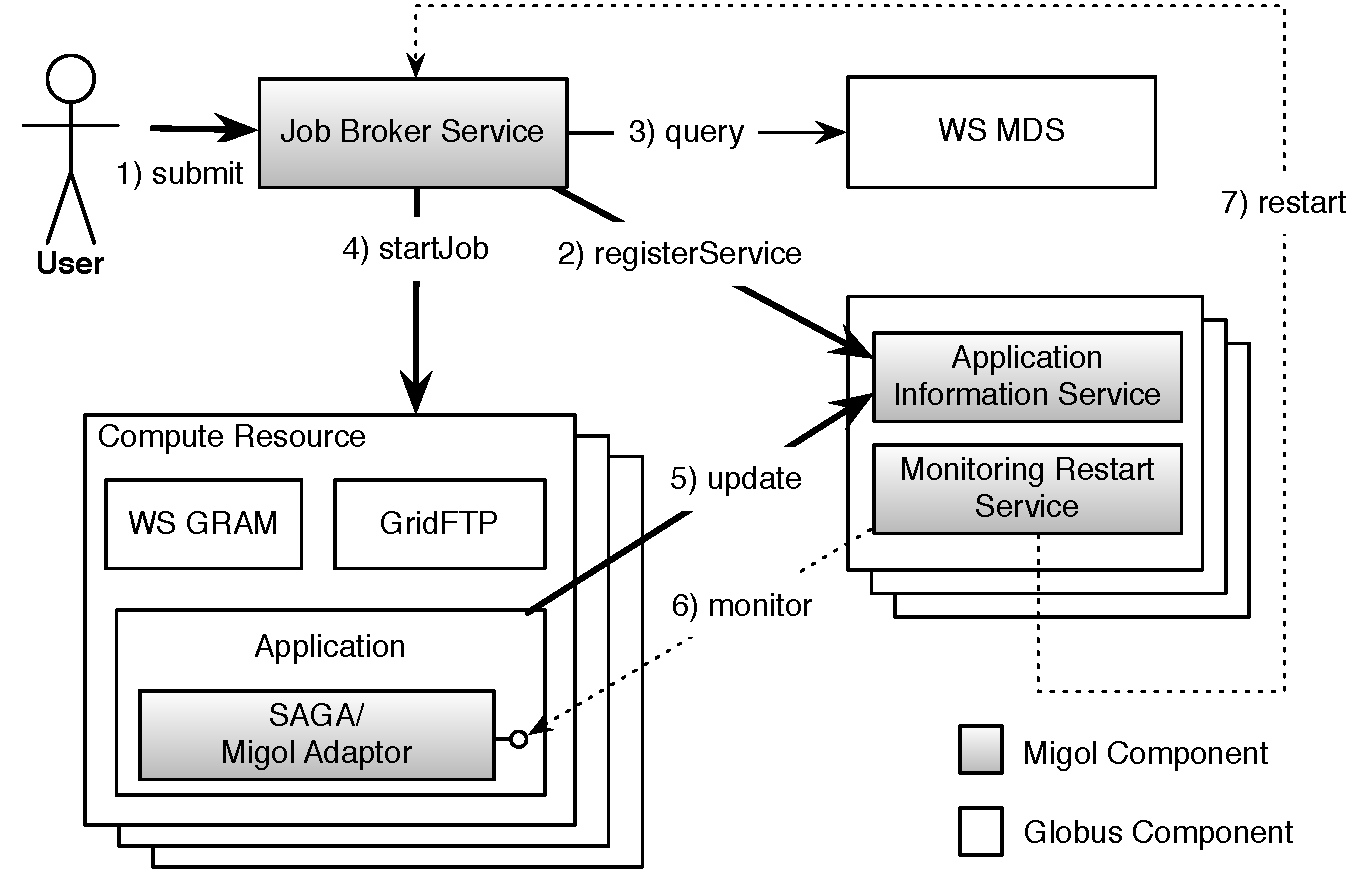
\includegraphics[width=0.5\textwidth]{migol_architecture}
 \caption{\small \bf Migol Architecture: Migol provides services for
 supporting the fault tolerance of Grid applications. Applications that are managed by
 Migol are transparently monitored and recovered in case of
 failures.\up\up
 }
 \label{fig:migol_architecture} 
\end{figure}           


Migol guarantees the correct and reliable exe\-cution of applications
or tasks even in the presence of failures. The framework is based on
the Globus Toolkit 4.  Figure~\ref{fig:migol_architecture} shows the
current Migol architecture and the interactions between the different
services.

The fundamental metadata model of Migol is the \emph{Grid Service
  Object (GSO)} schema, which defines a generic and extensible
information model for describing Grid applications.
%When an application is
%started, a Grid Service Object (GSO), which describedis created. 
A GSO stores all relevant information about an application: resource
requirements, the location of binaries and checkpoint files, global
unique identifier (GUID), etc.

Grid Service Objects containing the metadata of all running
applications are stored in the {\em Application Information Service
  (AIS)}.
% Applications can register and update service metadata, 
% such as files, machines etc.\ through Grid Services Objects. 
To avoid a single point of failure, the AIS is replicated using a ring-based
replication protocol, which ensures the data consistency
(see~\cite{Luckow:2008ys} for details).
%TODO plugin arch erläutern

% Figure~\ref{fig:migol_architecture} shows the current Migol architecture and
% the interactions between the different services.  
Applications are started using the {\em Job Broker Service (JBS)}
(step 1 in Figure~\ref{fig:migol_architecture}). Before a job
submission, the JBS must register the GSO of the application at the
AIS (step 2).  Resource discovery is performed through the WS
MDS~\cite{schopf06}  (step 3), which aggregates data of different services,
e.\,g.\ the Network Weather Service (NWS)~\cite{NWS99}.
Available resources are matched by the JBS according to the
requirements of the application. For execution of the application on
Grid resources, the JBS relies on a custom module, the Advance
Reservation Service, which is also capable of supporting reservation
of resources on top of the GRAM.

%  To better plan the execution of an
% application the JBS supports advance reservation. If the respective
% Grid environment is capable of handling reservations, the JBS
% negotiates a time slot with all suitable resources. All reservation
% offers are ranked based on a shortest expected delay
% strategy~\cite{Jeske:2007wj}.  For spawning of jobs on the selected
% resource, the Globus GRAM service is used (step 4).
%For conducting advance reservations and for job executions the
%\emph{Advance Reservation Service (ARS)} is used (message 4).
             
% To ensure the availability of the application state even in case of a failure, 
% checkpoints can be replicated to another site  using the \emph{Checkpoint Replication Service
% (CRS)}.  The CRS offers features such as the automatic discovery and selection of storage resources, 
% the management of the data transfer and the detection of new file versions. 
% The CRS uses an adaptive strategy to determine replication  targets respectively to select a replica for a
% job restart.

Migol provides several mechanisms for supporting the fault tolerance of 
distributed applications.
% Fault tolerance requires at least two basic mechanisms: failure
% detection and recovery. 
To detect failures, the \emph{Monitoring and Restart Service (MRS)}
periodically monitors all services registered at the AIS (step 6). 
In case the MRS discovers an inactive application, 
it initiates a restart respectively a migration using the JBS (step 7).

For recovery, Migol relies on application-level checkpointing, i.\,e.\
applications have to be written to accommodate checkpointing and
restart.  The checkpoint metadata maintained by the AIS must be updated by the application
each time a new checkpoint is witten  (step 5).

% To support an automatic recovery, Grid applications must be able to
% interact with the Migol infrastructure:
% \begin{compactitem}
%     \item The application must register checkpoint and job metadata with the infrastructure.
%     \item The infrastructure must be able to externally monitor the application.
%     %\item The infrastructure must be able to externally notify the application and trigger the saving of a checkpoint.
% \end{compactitem}  

Migol can be considered as GridCPR reference implementation for which
the SAGA-CPR package provides a well-defined, application-level
interface.  In addition, SAGA provides various other useful
abstractions, such as the File and RPC API, which ease the development
of distributed applications. The following sections describes how the
functionality of Migol can be seamlessly integrated with SAGA-CPR.


%  for which SAGA CPR aims, i.\,e.\
% The Simple API for Grid Applications (SAGA) provides a feature rich programing abstractions. 


\Section{SAGA Checkpoint Recovery API}

\up The SAGA API specification~\cite{saga_gfd90} defines not only the
core of the SAGA API itself, but also the mechanism to extend that API
by additional functional packages.  The SAGA-CPR API
Package~\cite{saga_cpr_draft} is such an extension, which is currently
an OGF working draft.  The SAGA-CPR package provides a clean
abstraction for starting, monitoring and recovery of
checkpoint-restartable jobs.
% The package was inspired by the GridCPR~\cite{gridcpr} architecture and Migol.
To support these use cases, applications can register checkpoint and job metadata with the infrastructure using this API. 
%Further, the API supports the starting of applications as well as the triggering of checkpoints and recoveries.

For the management of CPR Grid jobs, SAGA defines the \texttt{cpr::job} and \texttt{cpr::service} class (see 
Listing~\ref{lst:saga_job_start}). The handling of 
CPR jobs is similar to regular jobs: A job is defined using a job description. In contrast to normal jobs, 
CPR jobs require  two job descriptions -- one for starting and another one for restarting the application.
%Jobs are started using the job service (see Listing~\ref{lst:saga_job_start}). 
In addition to the normal job controls, CPR jobs can be queried for checkpoint metadata, 
and explicitly checkpointed or recovered. 
%Listing~\ref{lst:saga_job_start} shows the starting of a CPR enabled job.


\begin{lstlisting}[style=myListing, caption={\small \bf SAGA-CPR: Starting a Job}, float=t, label={lst:saga_job_start}]
saga::cpr::service js; 
saga::cpr::description jd_start;
saga::cpr::description jd_restart;
// fill out job description
...
// submit job  
saga::cpr::job job = js.create_job (jd_start, 
                                    jd_restart);
job.run ();
\end{lstlisting}

Listing~\ref{lst:saga_init_service} shows how applications can connect to the CPR infrastructure. During instantiation of the \texttt{saga::cpr::service} object the adaptor is able to register itself with the CPR backend. This step can e.\,g.\ be used to register a monitoring endpoint. Using the \texttt{saga::cpr::self} object an application can obtain metadata about the current job from the application.                                                                               
\begin{lstlisting}[style=myListing, caption={\small \bf SAGA-CPR: Initialize Migol Session}, float=t, label={lst:saga_init_service}]
saga::cpr::service service (saga::url 
    ("migol://flotta.haiti.cs.uni-potsdam.de:8443/wsrf/services/migol/AIS-JGroups"));
saga::cpr::self = service.get_self ();
\end{lstlisting}

Further, applications can use a checkpointing API to update checkpoint metadata at the backend. The SAGA-CPR API allows the hierarchically 
organization of checkpoint files. 
%and directories. Checkpoint directories are used to group checkpoints. 
% For example, parallel applications often write one checkpoint per 
% processor, i.\,e.\ in case of $n$ processors a CPR checkpoint
% would consists of $n$ files. Thus, a CPR checkpoint is designed as container 
% for multiple physical or logical files. 
Listing~\ref{lst:saga_chkpt_reg} illustrates 
the registration of a checkpoint file with the CPR framework.     
\begin{lstlisting}[style=myListing, caption={\small \bf SAGA-CPR: Checkpoint Registration}, float=t, label={lst:saga_chkpt_reg}]
saga::cpr::checkpoint remd_chkpt("remd_chkpt");
remd_checkpoint.add_file (saga::url 
  ("gsiftp://qb.loni.org/work/remd/chkpt.dat"));
\end{lstlisting}

\begin{figure}[h!]
    \centering
        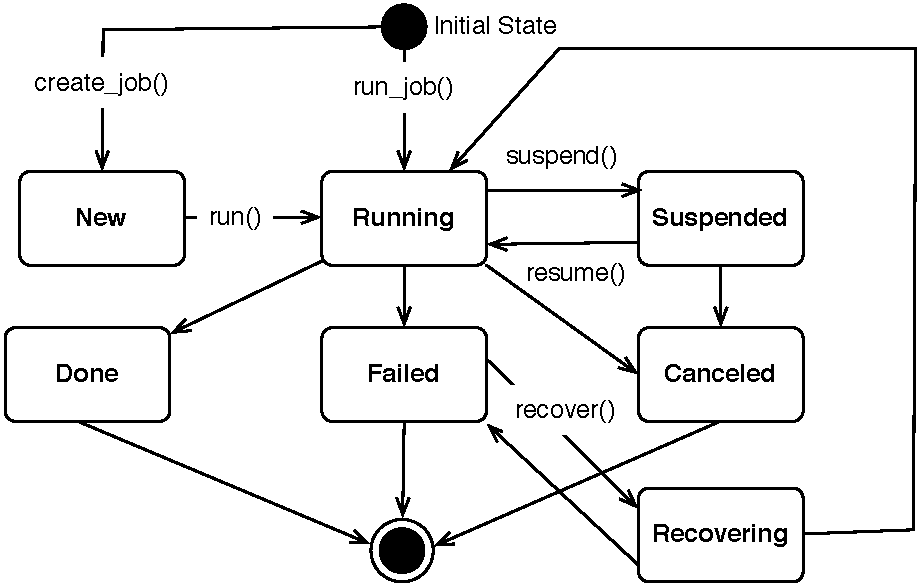
\includegraphics[width=0.43\textwidth]{cpr-statemodel.pdf}
    \caption{\small \bf SAGA-CPR State Model: The CPR state model introduces the recovering state. This state indicates that an automatic recovery attempt is  occurring.\up\up}
    \label{fig:cpr-statemodel}
\end{figure}
 

CPR jobs are subject to an extended state model. An application can query or subscribe to a job's state via the \texttt{cpr::job} object.      
Figure~\ref{fig:cpr-statemodel} summarizes the CPR state model. The CPR model extends the SAGA job state model by the new state \texttt{recovering}. This state
is used to indicate that the infrastructure is currently trying to restart a job. 
If this recovery attempt fails, the state of the application is permanently set to \texttt{failed}. 
The application must then deploy an application-level recovery schema in order to continue the execution. 


The Migol adaptor provides a compliant SAGA-CPR stack for the C++ reference implementation~\cite{Kaiser:2006qp}. 
A major building block is the application-level monitoring mechanism used to detect failures. 
To support the monitoring of arbitrary SAGA applications, a monitoring Web service is started 
by the Migol adaptor with the initialization of a \texttt{cpr::service} object. This 
service is implemented using the gSoap HTTP server~\cite{gsoap}.  The Monitoring Restart Service will 
periodically send heartbeat messages to the application's monitoring service.
% which periodically sends keep-alive messages to applications.                                                                             
% The URL of the service is registered at the Application Information Service where it can be obtained 
% by the monitoring service.

% A major building block for fault-tolerant system is failure detection. In general, fault detection is done by a monitor process, 
% which periodically sends keep-alive messages to applications. To monitor applications, the application must provide a communication endpoint.


Another critical aspect is the management of the application's
metadata. To ensure the recoverability of an application, metadata,
such as the job description and information about written checkpoint
files must be available even if the application failed. The Migol
adaptor relies on the AIS as the metadata backend. Every job is
associated with a global unique identifier (GUID).
%, which is initially created when an application first registers. 
All metadata belonging to an application can be stored or queried with
reference to the GUID.  The following information is propagated to the
AIS by the Migol adaptor:

\begin{compactitem}
\item The job description for starting and restarting of an
  application is mapped to the resource, service, and file profile of
  the Grid Service Object schema used by Migol. The registration of
  these information is done during the \texttt{create\_job()}
  operation.
\item The SAGA job state is mapped to the more comprehensive Migol
  model, which introduces additional states such as \emph{migrating}
  or \emph{pending}. All state transitions are directly propagated to
  the AIS. State queries, e.\,g.\ using the \texttt{get\_state()}
  operation, are always conducted against the AIS. The Migol state is
  accessible via the \texttt{state\_detail} metric of the job object.
\item After startup of the application, the monitoring endpoint,
  i.\,e.\ the URL of the Web service, is updated.
\item During the runtime, metadata about written checkpoint are 
  updated via the \texttt{cpr::checkpoint} object.
\end{compactitem}   
To ensure the availability of these information in case of a failure,
the AIS is actively replicated across multiple Grid nodes.

% MPI monitoring cannot be done without touch NAMD application In the
% following different implementation issues regarding the Migol SAGA
% adaptor are discussed.


\Section{Implementing Replica-Exchange Using SAGA}

\up \alnote{I removed parts of the SAGA introduction due to space
  reasons.}  \jhanote{I undid your removal, only because we need to
  emphasis the broad scope with SAGA} The \emph{Simple API for Grid
  Applications (SAGA)}~\cite{saga_gfd90} provides an easy-to-use
standardised API for developing a broad range of distributed
applications, including but not limited to loosely-coupled data and/or
task-parallel applications.  %The framework provides an standardized,
% easy-to-use API for applications to efficiently utilize Grid
% infrastructures.
In particular, SAGA offers an API for the management of
checkpoint-recoverable jobs and file transfers that can be used over
heterogenous distributed environment. Thus, SAGA is ideally suited for
encoding the orchestration logic of replica-exchange simulations.

\jhanote{Joohyun: Put in a paragraph or two of the main points of the
  how it is done here; maybe even discussing the ideas related to
  checkpointing, new jobs, MPI issues discussed etc. etc. Try to
  establish what is specific to the SAGA way of doing things from what
  is a general distributed computing problem/issue}

% This paper aims to demonstrate the efficient implementation armed with
% grid-enabled SAGA framework as well as fault-recovery SAGA-CPR Migol
% infrastructurure.
\begin{figure}[ht]
      \centering
          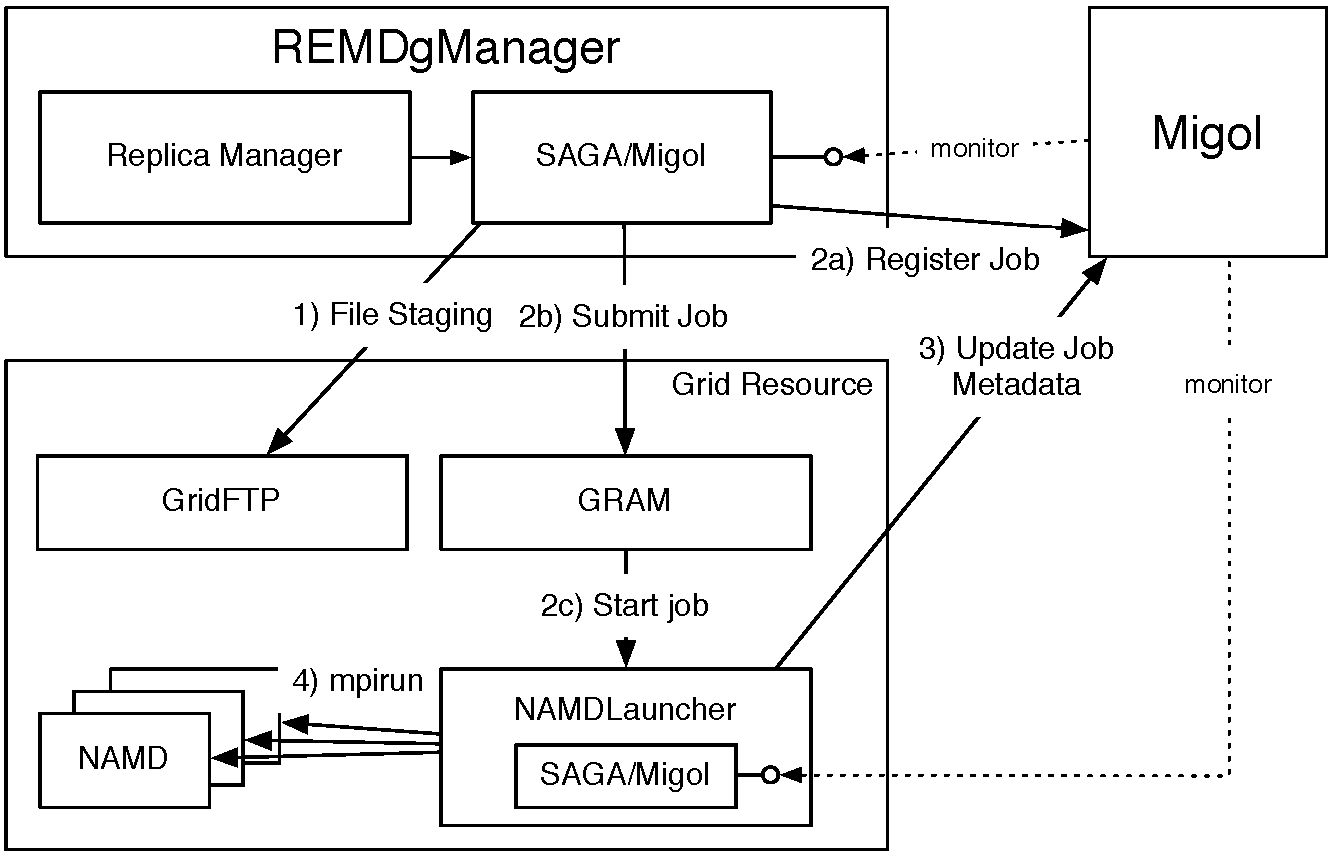
\includegraphics[width=0.5\textwidth]{REMDgManager-architecture.pdf}
          \up\up
          \caption{\small \bf Components of REMD-Manager: The main part of the
            framework is the replica manager. The manager orchestrates
            a set of replica processes using the SAGA/CPR API. The
            Migol infrastructure ensures that the REMD-Manager and all
            replica processes are monitored and recovered if
            necessary.}
            \up\up
      \label{fig:REMD-Manager-architecture}
\end{figure}
As illustrated in Figure~\ref{fig:REMD-Manager-architecture}, the
proposed framework comprises of three components: The task manager,
also referred to as \emph{REMD-Manager}, is deployed on the user's
desktop and provides the user interface for managing the overall REMD
run. The second component is Migol infrastructure that submits,
monitors, and, if required, recovers replica simulations.  The last
element is the task agent, the \emph{NAMD-Launcher}, that resides on
the High Performance Machines where MD simulations are carried
out. The NAMD-Launcher is triggered by the Grid job and is responsible
for spawning and monitoring of the MD
run. NAMD~\cite{Phillips:2005gd}, a highly scalable, parallel MD code,
is used for carrying out the MD simulation corresponding to each
replica run. It is important to mention that any other MD simulation
code could be used just as simply and effectively.

% The role
% of a task manager varies for achieving the best solution with
% different local environment at each HPC machine.  
% A REMD task manager and
% various parts gluing different components are mostly written with
% python scripts since SAGA-Python binding transparently exposes SAGA
% and SAGA-CPR/MIGOL APIs to simple but versatile Python.   

The \emph{REMD-Manager} is the core of the framework -- it is
responsible for orchestration of all replica processes, i.\,e.\ the
parameterization of replica tasks, file staging, job spawning and the
conduction of the replica-exchange itself. The component heavily
relies on the SAGA File and CPR API as well as the Python bindings for
implementation of the RE
logic. Listing~\ref{lst:python_saga_chkpt_reg} illustrates the
application sequence of a RE simulation.
                                  
\alnote{I am really not sure about this code snippet. It somehow
  represents the logics - however I am not sure whether it is worth
  the space.} \jhanote{I agree, that as written it is not very
  effective. Also, since it does not show the exchange and thus the
  reader does not see how ``distributed'' and ``local'' exchanges are
  handled equally simply. Can we i) use psuedo-code to highlight this?
  ii) mention where the reader can get the actually code?. We should
  definitely do point ii) and possibly point i)}
\begin{lstlisting}[style=myPythonListing, float=t, caption={\small \bf
REMD-Manager: Replica Orchestration},
label={lst:python_saga_chkpt_reg}]
# initial job launching       
...
# main replica exchange loop                    
while num_exchanges < total_num_exchanges: 
   irep=0
   while rep_id < numReplica-1:
     # pairwise monitoring of the job state
     job1 = rep_list.jobs[rep_id]
     state1 = job1.get_state()
     job2 = rep_list.jobs[rep_id+1]
     state2 = job2.get_state()
     if (str(state1) == "Done" and str(state2)=="Done"):
         # conduct exchange
         ...
         # restart both replicas  
         for i in rep_id, rep_id+1:
             # transfer files
             ...
             # restart replica
             js = saga.cpr.service()
             jd = create_job_description(i)    
             job = js.create_job(jd, jd)
             job.run()
             rep_list.jobs.append(job)
         num_exchanges = num_exchanges + 1
     irep = irep + 2
\end{lstlisting}

% The application utilizes the SAGA-CPR
% API and the underlying Migol infrastructure to efficiently and
% reliable manage replica
% processes. Figure~\ref{fig:REMD-Manager-architecture} illustrates the
% architecture of the REMD-Manager.  

% Each replica-exchange step consists of many replica runs  at 
% different temperatures. 
% Each job corresponds to one replica run of NAMD 
% with an assigned temperature.  

Depending on the number of configured processes $n$, the REMD-Manager
starts initially $\frac{n}{2}$ pairs of replicas.  Each replica
process is assigned a different temperature. Before launching the job
the REMD-Manager ensures that all required input files are transfered
to the respective resource. For this purpose, the SAGA File API and
the GridFTP adaptor (step 1 in
Figure~\ref{fig:REMD-Manager-architecture}) are used.  The replica job
is then submitted to the Grid resource using the CPR API and
Migol/GRAM (step 2a-2c). Migol ensures that the the job description of
each replica is stored within the Migol backend to ensure a later
recovery. Globus GRAM is used to start the application.
                                               
To integrate NAMD with the SAGA/Migol infrastructure a SAGA based task
agent -- {\it NAMD-Launcher}, is used.  This agent is responsible for
updating the metadata of the application, i.\,e.\ the state,
monitoring endpoint and the URLs of newly written checkpoints at the
Migol backend.  The agent then launches the actual NAMD job using
MPI. During the entire runtime the replica process is monitored by
Migol using the monitoring endpoint of the NAMD launcher. This
NAMD-Launcher enables the flexible orchestration of multiple NAMD jobs
through the REMD-Manager without modification of the NAMD source
itself.

% After all replicas have been successfully completed,
% the exchange step is conducted, i.\,e.\ the REMD-Manager determines
% new parameters for all replica tasks, stages the required files and
% relaunches all jobs.

If a pair of replica jobs finishes, the new replica parameters such as
the new temperature are determined by the Metropolis scheme.  Both
jobs are then relaunched using the mechanisms described above.

SAGA allows the simple decoupling of the REMD application logic from
the underlying Grid infrastructure. Using the Migol adaptor, the
application can benefit from features, such as the automatic
monitoring and the transparent recovery of failed tasks.  \jhanote{May
  want to replace or remove: At the same time, SAGA allows the
  application to easily utilize other infrastructures in conjunction
  to or as replacement to Migol.}

% The current parameterization of each replica is
% stored within a list object and can be referenced by the
% \texttt{replica\_id}. 
% For each replica job different metadata, such as the
% working directory, the used configuration file, the temperature
% etc., is maintained by the REMD-Manager.  This data is used by the REMD-Manager to
% transfers all required files to the respective resource using the SAGA
% File API and the GridFTP adaptor (step 1 in Figure~\ref{fig:REMD-Manager-architecture}). 

% SAGA APIs and SAGA-CPR Migol infrastructure allow a user to build
% his/her own implementation of REMD adaptively considering the
% limitations of available resources.  That aspects comes from the
% high-level abstraction of SAGA and flexible implementation of
% Replica-Exchange as well as fault-recovery with SAGA-CPR Migol.  For
% example, one simple scenario is to assign a REMD manager in charge
% of a job submission/monitor/fault-recovery.  Each job corresponding
% one replica run with a assigned temperature is sent to HPC machine
% as a parallel MPI job by the manager and overall job execution and
% fault-recovery are monitored by the manager.  The following snippet
% shows the part of the code written with python for the REMD manager
% showing creation and submission of a job corresponding to each
% replica.
                                             
% \jhanote{I say we put a few snippets of code here}

% Joohyun's old code
% while 1:
%     js = saga.cpr.service() 
%     jd_start = saga.cpr.description()
%     jd_restart = saga.cpr.description()
%     # job description for each replica stored in the configuration file is retrieved
% ...
%    #checkpoint file registration
%    saga.cpr.checkpoint remd_chkpt("remd_chkpt");
%    remd_checkpoint.add_file (saga.url ("gsiftp://qb.loni.org/work/remd/chkpt.dat"));
% ...   
%    #job submit
%     new_job = js.create_job(jd_start, jd_restart)
%     new_job.run()
%     REMDjobs.append(new_job)     

% old code's second version
% # loop n replica-exchange steps  
% for i in range(0, n):     
%     # spawn jobs
%     for replica_id in range(0, num_replicas):
%       js = saga.cpr.service()
%       jd = create_job_description(replica_id, replica_info)    
%       replica_job = js.create_job(jd_start, jd_restart)
%       replica_job.run()
%       replica_list.append(replica_job)
%      
%     # wait for termination of jobs
%     for replica_id in range(0, num_replicas):     
%         replica_list[replica_id].get_state()
%         if (state=="Done"):                          
%             #obtain result of replica process
%             energy[replica_id] = get_energy(replica_id)
%  

\Section{Experiences with REMD}
\label{sec:exp}       
        
\up To evaluate the performance of the REMD-Manager several
experiments have been conducted on LONI Grid~\cite{Allen:2003xy}. The
REMD-Manager is used to deploy tasks to three LONI clusters: QueenBee,
Eric and Poseidon.  \jhanote{I think we want to say REMD simulations
  have been deployed on three LONI Linux Clusters? Not the managers
  themselves -- which I think sits on users desktop...}
\alnote{adjusted that - should i change figure 4 too, although for the
  measurements all jobs have been launched from QB. There are some
  firewalls which limit the desktop experience.}
 
QueenBee, which is both a LONI and a TeraGrid resource, is the largest LONI
machine and has a peak performance of over 50 TFlops.
Figure~\ref{fig:saga-taskfarming} gives an overview of the experiment
setup.

\begin{figure*}[t]
    \centering
        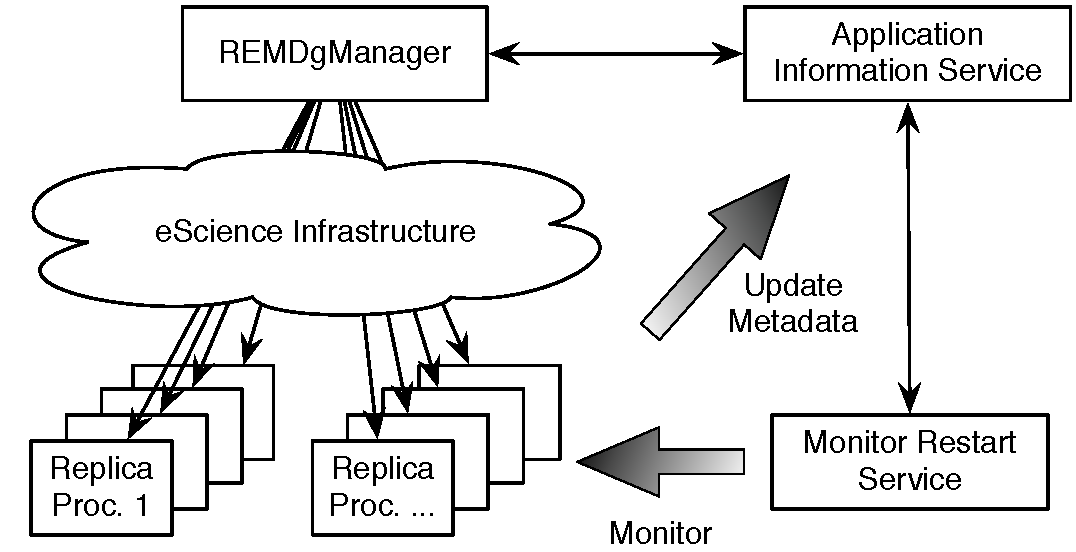
\includegraphics[width=0.7\textwidth]{saga-taskfarming}
        \caption{\small \bf Fault-Tolerant MD Simulations: The
          REMD-Manager orchestrates a set of distributed replica
          processes using the SAGA API. All processes synchronize
          important metadata with the Migol infrastructure. Migol then
          actively monitors all processes and ensures that, even in
          the presence of failures, all task are eventually
          completed.\up\up}
    \label{fig:saga-taskfarming}
\end{figure*} 
The main objective of the experiments is the quantification of the overhead, 
which Migol-enabled applications, such as the REMD-Manger, must be expected.
Scientific results obtained from using this infrastructure will be 
reported elsewhere.
% In particular, . This overhead is caused by the necessary
% interactions with the Migol backend, in particular for job submission,
% registration of metadata and active monitoring.
\begin{figure}[ht]
    \centering
        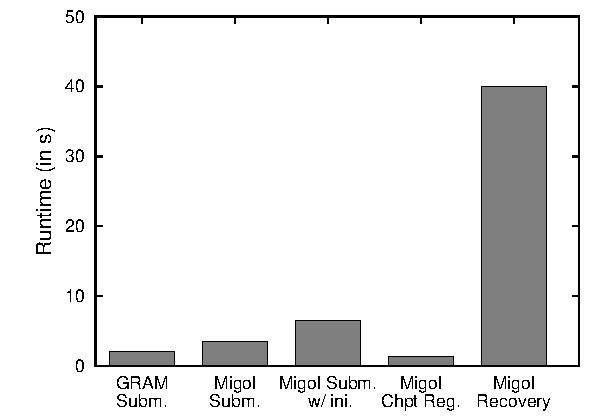
\includegraphics[width=0.45\textwidth]{performance/perf_submission.pdf}
    \up
    \caption{\small \bf SAGA/CPR Migol Adaptor Overhead}
    
    \label{fig:performance_perf_submission}
\end{figure}           
Figure~\ref{fig:performance_perf_submission} gives a response time
analysis of important CPR API operations in comparison to their non
fault-tolerant counterparts. Since each replica exchange step involves
the relaunching of both replica jobs, the spawning of remote tasks is
a particular critical operation for the REMD-Manager.
% step {\bf n} replica processes
% must be launched and monitored \jhanote{I am not sure I understand the
%   previous sentence completely. Need to discuss} 
To assess the overhead, the submission time of a single NAMD task
using SAGA-CPR/Migol was initially assed. The experiment showed that a
CPR/Migol job submission is on average 2\,seconds slower than a normal
GRAM submission. This overhead is mainly attributable to the
additional metadata registration operation at Migol's AIS. However,
for jobs that run on the order of hours, a couple of seconds overhead
is effectively negligible.

Further, the Migol adaptor showed some additional initialization
overhead.  The overall runtime of this simple NAMD submission task
including the initialization was 6.5\,sec (bar 3 in
Fig~\ref{fig:performance_perf_submission}), about 4.5\,sec slower than
the GRAM submission task. This overhead can be attributed to the
initialization operations for setting up the HTTP server as well as
the conduction of several metadata updates on the AIS. Since this
initialization only occurs once after the startup of the REMD-Manager,
this overhead is acceptable.
                                                                                                                    
In addition to the job submission, we investigated how the runtime of
a replica process is effected by Migol's active monitoring mechanism
and the required checkpoint registration.  To evaluate the runtime
overhead, a NAMD job with 1000 steps was started with and without
Migol support.  Further, monitor intervals between 20\,s and
2\,minutes have been chosen to study the effect of the monitoring
period on the NAMD runtime.  The update interval for checkpoint
metadata was set to five minutes.  Since the time measured for a
checkpoint update operation was on average 1.3\,seconds, we do not
expect this to be a critical factor.  The runtime of the NAMD job on
QueenBee without CPR/Migol amounted to 21.3 minutes.  At worst a 1
minute overhead was observable with a monitoring interval of
20\,s. With a less eager monitoring period almost no overhead was
detectable -- the runtime overhead measured with a 2\,minute
monitoring interval was 10\,s. This time is only slightly higher than
the variance of the typical NAMD runtimes.
% During
% this 21\,minute NAMD run the overhead average to 20\,s and thus only
% amounts to about 2\%.
% \begin{figure}[htbp]
%     \centering
%         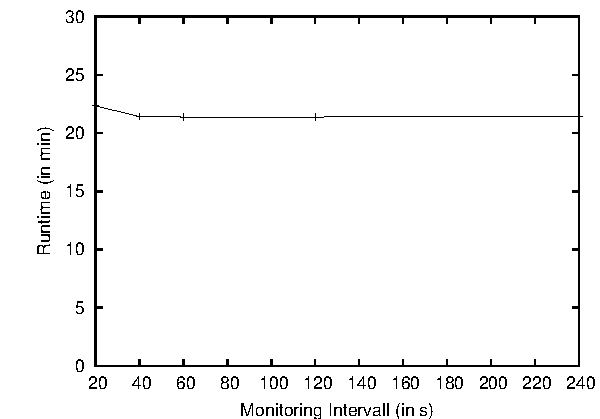
\includegraphics[width=0.5\textwidth]{performance/perf_monitoring.pdf}
%     \caption{\small \bf Analysis of Monitoring Overhead}
%     \label{fig:performance_perf_monitoring}
% \end{figure}     

Further, we evaluated the performance of the REMD-Manager.  
The REMD-Manager was configured to run a REMD simulation with 
2 to 16 replica processes and 16 replica-exchange
steps. To stress test the Migol infrastructure very short NAMD tasks
with only 100 steps have been used. Table~\ref{tab:app_stats}
summarizes the REMD configuration used. The runtime of a REMD simulation depends 
to a great extend on the queuing time at the local resource 
management system. During the measurements it was ensured that jobs became 
active right away; however, small queueing delays could not always be avoided.

\begin{table}        
    \centering
	\begin{tabular}{|p{5cm}|l|}
          \hline
          %Molecular Dynamics Code &NAMD\\ \hline
          Number of NAMD steps &100\\ \hline 
          Number of NAMD processes &16\\ \hline 
          Required staging files/size &6\,files/10\,MByte\\ \hline
          %Runtime of a single NAMD task (QueenBee) &2\,minutes\\ \hline   
          Number Replicas &2-16 \\ \hline
          Number of Replica-Exchanges \jhanote{See caption for Q} &16\\ \hline
          %Total Runtime: &??   \\ \hline
	\end{tabular}
	\caption{\small \bf REMD Application Characteristics\label{tab:app_stats}
          \jhanote{Is 1000 the the total number of exchanges or the
            number of exchanges that a single replica will undergo?}
          For completeness we should probably mention the temperature
          range over which simulations were performed}
          \alnote{Each replica process (NAMD simulation) will conduct 
          100 steps (referred to as NAMD steps in the table). This 
          will be repeated 10 times (number exchange steps) with 
          different temperatures.}         
          \alnote{Maybe we should remove this table and put the not mentioned information 
          into the text}
          \up\up
\end{table}   

\begin{figure}[htb]
    \centering
    \hspace*{-20pt}
        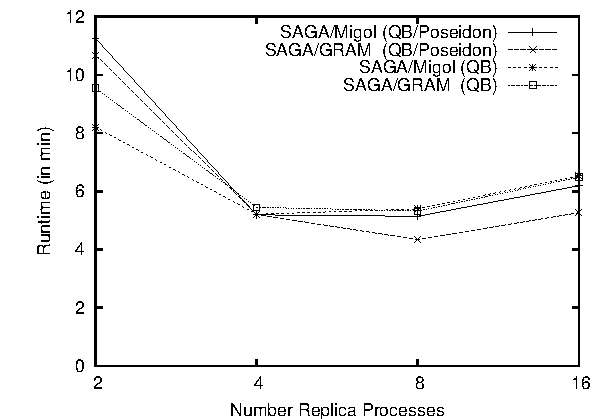
\includegraphics[width=0.5\textwidth]{performance/perf_remd.pdf}
        \caption{\small \bf REMD Runtime Analysis: The time (in minutes) that it
          takes to complete 16 replica exchanges; each replica
          runs for 100 steps, before attempting an exchange with a
          sister-replica. The overhead of the Migol is about 2\,minutes. \jhanote{need some further clarity}     
          \alnote{figure not correct yet - just found a bug in the REMD-Manager... starting over}
          \up\up}
    \label{fig:performance_perf_runtime}
\end{figure}     

\alnote{This must be reworked with the new results!}
Figure~\ref{fig:performance_perf_runtime} illustrate the results of
this evaluation. Since the overall number of replica exchange steps remained constant,
the runtime decreases the more replica processes are available. However, with more than 8 processes a slight increase 
of the runtime is observable. 
% This is a result of the sequential overhead which proportional 
% grows with the number of replicas: 
The more replica processes, the more exchanges the REMD-Manager must handle
concurrently. Each exchange requires the re-staging of 6 files with the size of 12\,MB -- this transfer alone typically 
requires 5-10\,s within LONI. Due to the small problem set computed by each 
replica (only 100 NAMD steps, which require 35\,seconds computation time on QueenBee), 
this bottleneck becomes very evident. However, in more realistic scenarios with larger problem chunks
this issue will be avoided.  


The results also show that an overhead caused by Migol is hardly measurable. Per average, the Migol adaptor showed 
about 15\,seconds runtime overhead, which correlates
to earlier findings depicted in Figure~\ref{fig:performance_perf_submission}.


% The REMD-Manager sequentially stages and starts all jobs.  Especially for
% short-running NAMD tasks as used for this experiment this overhead
% amounts to an over-proportional part of the runtime. This can be
% improved in the future by supporting parallel launches and file
% staging activities.  Further, all replica jobs are run through the the
% PBS queue of the cluster systems.  In general, jobs on QueenBee became
% active right away and thus, the queuing time can be neglected in this
% scenario.  The overall overhead observed from CPR/Migol in contrast to
% a SAGA/GRAM submission corresponds to the result depicted in
% Figur~\ref{fig:performance_perf_submission}.
% the regular replica-exchange schema, i.\,e.\ 

Further, the REMD-Manager has been successfully deployed across
multiple Grid nodes. During this distributed run 1/4 of the processes have been 
allocated to the smaller Poseidon machine, while the remainder stayed on QueenBee.
Using this configuration, a slightly better performance than the QueenBee only run
is noticeable. However, especially the smaller machines showed long queuing times 
leading to high variance in the overall response
times. In our scenario, the response time rapidly increases when we tried to allocate 
more processes on Poseidon. 
% Especially for short-running tasks as used for this test this 
% overhead is significant. 

\kimnote{However, this simple scenario faces high overhead since each
  job is submitted to the local scheduler in many cases. \it
  Shantenu, may be you can write here another scenario we discussed
  as an alternative to the simple scenario we are testing.  If I can,
  I will try, too }            
\alnote{I added some remarks towards a enhanced scenario as result of the measurements}  

Further, the reliability capabilities of the proposed framework have
been extensively researched by inserting of faults into the
systems. In our scenario, we killed selected replica processes and
measured the time required by Migol to restarting the system.  Due to
the selected monitoring intervall of one minute and failure threshold
of 2 tries, the failure detection time averages to 2.5\, minutes.

As shown in Figure~\ref{fig:performance_perf_submission} the recovery
time required for the restart of the job is about 42 seconds. This is
mainly caused by the complex interactions conducted by the Migol
backend (cmp. section~\ref{sec:migol}): The monitoring service
initializes the restart at the JBS.  A major performance penalty is
the delegation-on-demand mechanism required to obtain the credential
of the user from the AIS -- this procedure demands the creation of a
public-private key pair, which is very costly. The JBS then discovers
and allocates resources.  The job start itself is conducted via the
reservation module of the JBS. In contrast to the GRAM, this module
supports advance reservation based on a dynamic resource manager detection
mechanism. In particular this feature is currently associated with 
some overhead.

% , the ARS is
% not bound to a single Grid site, i.\,e.\ if allowed by the
% administrator it is able to conduct reservation respectively job
% starts at any resource in the Grid. Local resource management systems
% are detected during the runtime of the job. However, this feature is
% associated with some overhead in contrast to a simple GRAM submission.

% \begin{itemize}
%     \item The  Migration Service is called - the services verifies the state of the application and tries to trigger a checkpoint
%     \item Job Broker Service: verifies state of resource job was
%       allocated before. This requires some interaction with the
%       MDS. In addition bandwidth information etc. are acquired
%     \item restarts the job at the respective resource. Due to
%       architectural reasons Migol jobs are restarted through the
%       Advance Reservation Service. It's most noted feature in
%       contrast to the GRAM is the support for advance
%       reservation. In contrast to the GRAM, the ARS is not bound to
%       a single Grid site, i.\,e.\ if allowed by the administrator it
%       is able to conduct reservation respectively job starts at any
%       resource in the Grid. Local resource management systems are
%       detected during the runtime of the job. However, this feature
%       is associated with some overhead in contrast to a simple GRAM
%       submission.
% \end{itemize}   

While these results show that SAGA/CPR in conjunction with Migol
incurs some overhead, we think that this is acceptable compared to the
benefits a fault-tolerant, self-healing infrastructure offers. In
addition, it must be noted that further simple yet effective
optimizations are possible. For example, by directly restarting jobs
via the GRAM service a lot of the overhead caused by the dynamic
discovery mechanisms incorporated within the JBS services can
be avoided. Further, we will evaluate possibilities to decouple
the dispatching of replica runs from allocation of cluster resources 
to avoid long queuing delays. Systems, 
such as Falkon~\cite{1362680} or the Condor Glide-In~\cite{citeulike:291860} 
mechanism provide the possibility to acquire a chunk of resources 
from the resource management systems, which can
then be used to dispatch short tasks.

% \jhanote{This might be right place to talk about
%   Condor-Glidein, or an agent that provides block queue reservation
%   over multiple processors}. 

% Some comments with respect to solved REMD problem: about 17 MB data
% to transfer for a migration

% The REMD-Manager was functionally tested on the LONI Grid. The following aspects are from interest:
% \begin{itemize}
%     \item \textbf{Speedup}: This test determines how much faster the Grid-enabled replica-exchange algorithm is in comparison  to a sequential and/or a not Grid-enabled version.
%     
%     \item \textbf{Migol Overhead}:  During this test the overhead imposed by the Migol framework in comparison to a traditional SAGA/Globus infrastructure is evaluated. This overhead is mainly caused by the application-level monitoring, but can also be attributed to the necessary interaction with the Migol backend, e.\,g.\ for the registration of checkpoints. The following  metrics are evaluated:
%     \begin{itemize}
%         \item percentage overhead in runtime dependent on the monitoring interval
%         \item runtime overhead of Migol job submission and meta-data registration. 
%     \end{itemize}                                                           
%     
%     \item \textbf{Fault Injection Test:}  During this test, the functionality of the Migol framework is assed by introduction of different faults during the application run, e.\,g.:
%     \begin{itemize}
%         \item the failure of one or more worker nodes, or
%         \item the failure of the master node.        
%     \end{itemize}                       
%     During the test the correctness of the Migol framework and application is verified. In addition, the following metrics are determined:
%     \begin{itemize}
%         \item failure detection and recovery time
%         \item application runtime in correlation to the number of faults
%         \item recovery time versus false failure detection rate dependent on the monitoring intervall.
%     \end{itemize}
%                                                                                  
%     \item \textbf{Scalability test}: This test determines up to how many worker nodes the infrastructure is able to scale.
%     \item \textbf{Extended statistical analysis}: This evaluation determines the failure rates during REMD simulation runs. Further, it will be assessed how many of these real life failures can be detected and recovered by Migol. 
%                                                 
%     \alnote{The last two aspects should go due to timing reasons into the Phil Trans paper.}
% \end{itemize}
     

\Section{Related Work}

% TODO AM: add some SAGA-CPR background

\SubSection{Previous CPR Efforts}

\up
\jhanote{This might have to be commented out: Checkpointing and
  rollback recovery is widely used in Grids. For example, the
  Condor/PGRADE system~\cite{DBLP:conf/eagc/KovacsK04} consists of a
  checkpointing mechanism for PVM applications and uses
  Condor-G~\cite{citeulike:291860} for scheduling.  While PGRADE
  emphasises an integrated user-level checkpoint approach, we believe
  that this approach is not suitable for a heterogeneous Grid
  landscape. Further, the framework does not ensure the
  fault-tolerance of the service infrastructure sufficiently.}
                                 
% Condor-G~\cite{citeulike:291860} allows the management of multi-site
% computations.


% Several frameworks for high-throughput computing and task farming
% exist: Nimrod-G~\cite{buyya00nimrodg} is a specialized framework for
% task farming. The framework provides a user interface for describing
% task farming applications. For remote execution of jobs Globus is
% used. While the user interface is very suitable for parameter studies,
% more demanding problems such as REMD simulations require a further
% application-level integration.

% The Legion~\cite{689541} Grid middleware provides a object-oriented
% programing model, which allows the simple instantiation of distributed
% tasks. While the provided abstraction is useful for developing Grid
% applications, it relies on proprietary protocols and is not compatible
% with OGSA-based service-oriented Grids.

% Nimrod-G and Legion as also most Grid resource management systems,
% such as Condor-G~\cite{citeulike:291860} and GridWay~\cite{Montero05},

Several frameworks for high-throughput computing and task farming
exist, Condor-G~\cite{citeulike:291860},
Nimrod-G~\cite{buyya00nimrodg}, and Legion~\cite{689541} to name a
few. These provide basic fault tolerance support by automatic
re-scheduling failed tasks. Advanced features such as the management
of checkpoints however, are not supported. Further, these frameworks
rely on a very simple failure detection mechanisms -- usually by
simply polling the job state at the Globus gatekeeper. This allows the
detection of some errors, but application-level failure detectors as
used by the Migol/SAGA library can detect much more complex
errors. For example, especially parallel applications can fail quite
inconsistently: in the best case the application aborts, at worst the
application hangs indefinitely. These kind of failures are not visible
at Grid resource management system level.

\jhanote{This will have to be commented out: Further, these frameworks
  or schedulers focus on individual aspects, e.\,g.\ Nimrod-G focuses
  on task farming or GridWay on meta-scheduling. Migol aims to provide
  an overall autonomic, self-healing infrastructure, which addresses
  the fault tolerance of Grid applications and the infrastructure
  itself.}

At the level of related application programming interfaces for
checkpointing, proprietary interfaces are dominant. This is because
applications most often rely on application level checkpointing, and,
related, perform also their own checkpoint management (checkpointing
policies, frequencies, dependencies, staging etc).  
\alnote{Should we remove this from here - this is already mentioned now at the 
beginning.}
The Open Grid Forum's\footnote{\texttt{http://www.ogf.org}} GridCPR group (Grid
CheckPoint and Recovery) made an early attempt to describe a generic
CPR architecture, and to define a generic CPR API, which would support
applications to manage their complete checkpoint/recovery life
cycle~\cite{ogf_cpr_arch}.  Based on that architecture, and on a set
of CPR use cases~\cite{ogf_cpr_uc}, the SAGA group in OGF defined the
CPR API package~\cite{saga_cpr_draft} (work in progress), whose
implementation is described in this paper.  The rendering of the CPR
API in the SAGA API framework allows (a) to seamlessly combine CPR
operations and other high level Grid programming abstractions provided
by SAGA, and (b) to abstract from the actual implementation of the CPR
mechanism.  The CPR API which has been demonstrated with the Migol
fault tolerance framework, can work just as well with, for example,
the XtreemOS system level checkpointing
capabilities~\cite{xtreemos_cpr}.


\SubSection{Other Distributed RE simulations}
% \jhanote{We need to compare our approach with i) WISDOM and ii)
%   Folding@HOME}             

\up
Several project, such as Folding@home~\cite{folding} and
Wisdom~\cite{wisdom}, rely on distributed infrastructures for
computational biology and chemistry. While
Folding@home~\cite{PhysRevLett.86.4983} utilizes a somewhat similar RE
algorithm\footnote{Folding@Home~\cite{PhysRevLett.86.4983} is parallel
  replica dynamics but that is a special case of replica-exchange;
  when a certain event happens, there is a need for coordination
  amongst ALL replicas. We should maybe point this out, but I think it
  is fair at this level of detail, to consider folding@Home to be in
  the same application class to effectively parallelize simulations}
it is based on BOINC~\cite{1033223}, a cycle scavenging
infrastructure.

%   \kimnote{Is this true? I know early attempts with Folding@home only
%     focused on parallel replica dynamics that does not need exchange!
%     They only get independent run results limited to the short time,
%     and use those large number of simulations for predicting kinetics,
%     I think}

The Wisdom project utilizes the EGEE infrastructure for molecular
docking simulations used e.\,g.\ for evaluation of drugs. While this
application has a similar high throughput characteristic, the project
is currently tied to the gLite~\cite{glite2008} Grid middleware.

% In contrast, general, multipurpose Grids as the TeraGrid, which
% provide a dedicated runtime environment for applications with
% different characteristic, e.\,g.\ loosely coupled, tightly coupled and
% data-intensive applications, desktop Grids rely on volunteers. This
% kind of environment is only suitable for loosely coupled
% applications. Multipurpose Grids have several advantages: Issues as
% trust and security are well researched. Further, it is possible to run
% larger application chunks. The REMD manager splits an scenario into
% multiple parts -- each part can be represented by a MPI application
% utilizing up to 32 nodes. \jhanote{needs refinement will do}
% \kimnote{Yes, this is MPI enables and there is no limitation on the
%   number of nodes!}

In contrast to Wisdom and Folding@home, our approach is not restricted
to a specific Grid middleware -- by utilizing the SAGA standard the
REMD manager can easily utilize resources managed by different
general-purpose Grids.  SAGA provides a well-defined abstraction,
which is capable of handling both scenarios. Using this approach the
application can easily used with different middleware platforms,
Folding@home could then be deployed on a BOINC infrastructure as well
as on a multipurpose Grid, such as TeraGrid.

\alnote{Should we add some details regarding the scientific results of
  WISDOM and Folding@home and how they differ from our REMD with NAMD?
  Or are we just comparing the Grid infrastructure?}  \jhanote{In
  response to immediateley preceeding alnote, IMHO we don't need to
  address scientific results, but will just say the ``size of the
  problem'' that can be studied is limited}

% In addition, SAGA provides many benefits for applications.  SAGA
% offers a feature rich programing abstractions, which can be used in
% conjunction with the fault-tolerant Migol framework, but also with
% other Grid middleware platforms.
% 

%%------------------------------------------------------------------------------
\Section{Conclusion and Future Work}

\up
We have developed a fault-tolerant framework that implements a
commonly occuring application usage pattern -- a loose-coupling of
multiple tightly-coupled applications -- whilst being general purpose
and extensible to different usage patterns, deployment scenarios and
specific simulation codes.

The fault-tolerant framework used to implement RE simulations in a
production environment is created using the distributed programming
interfaces provided by SAGA and its coupling to Migol to provide
fault-tolerant features.  SAGA provides a middleware-independent,
programing abstraction for distributed environments. RE simulations
utilize the new SAGA-CPR API, which provides an ideal interface for
Grid applications to interface with a checkpoint-recovery
infrastructure, such as Migol. Using the newly developed SAGA adaptor
for Migol, any SAGA application can re-use Migol's fault-tolerant
services for monitoring and recovery.  The application developer is
not required to provide any special code, solely the Migol adaptor
must be configured.  The framework has strong self-healing
capabilities: critical services, such as the Application Information
Service (AIS) are able to automatically detect failures and
reconfigure themselves, and thus addresses common failure modes in
distributed environments without user interactions.
%fault tolerance of Grid applications by handling common
%failures in Grid applications transparently without user interactions.
In case of failures, e.\,g.\ a node-crash, applications are
automatically restarted from the last saved
checkpoint. % Migol is designed with focus on fault tolerance.

In contrast to other RE implementations on distributed
simulations it is critical to note and emphasis the general usability
and extensibility of our approach -- across different infrastructure,
across a range of scientific applications and usage patterns (such as
the multiple variant of the RE).

\jhanote{In future work, we need to mention that we are deploying this
  infrastructure on a real distributed system (LONI) and are using it
  to study the binding interactions of peptide-RNA (Joohyun, would you
  agree?). We will report on the specific science results obtained
  using this approach in publication TBD but most likely Phil Trans of
  Royal Soc A}

%\Section{Acknowledgements}
\begin{acknowledgement}
  \up This work would not have been possible without the efforts and
  support of the wider SAGA team, especially Hartmut Kaiser, Ole
  Weidner and Joao Abecasis. We also thank Daniel Katz for hosting AL
  at the CCT, when this work was conceived.  Important funding for
  SAGA specification and development has been provided by the UK EPSRC
  grant number GR/D0766171/1 (via OMII).  SJ acknowledges the
  e-Science Institute, Edinburgh for supporting the research theme,
  ``Distributed Programming Abstractions''.  This work has also been
  made possible thanks to the internal resources of the Center for
  Computation \& Technology (CCT) at Louisiana State University and
  computer resources provided by LONI.
\end{acknowledgement}


\bibliographystyle{IEEEtran}
% \bibliographystyle{plain}
\bibliography{saga,literatur}
\end{document}


%TODO Future Work

%Migol provides an integrated solution for the management of data and
%compute resources.

% A main limitation of current Grid infrastructures is the restricted availability of 
% precise resource information. Managing this information uncertainty is difficult and often leads to
% a trial-and-error approach. For example, a transfer service cannot 
% differentiate between a harddisk failure and a transient network failure. While a retry 
% will resolve a transient failure, in case of a harddisk failure this approach will very likely not be successful.
% An adaptive strategy for tuning fault detection timeouts is therefore essential to achieve a 
% sufficient reliable fault detection while maintaining an acceptable performance.        

% Granularity of SAGA API not always well suited for Grid service interactions.
%%------------------------------------------------------------------------------     




% \begin{abstract}   {Grid Computing, Task Farming, SAGA, Migol}
% A major challenge in a dynamic Grid with thousands of machines connected to
% each other is fault tolerance. The more resources and components involved, the
% more complicated and error-prone becomes the system. 
% Migol~\cite{schnorLuckow08} is an adaptive Grid middleware,
% which addresses the fault tolerance of Grid applications and services 
% by providing the capability to recover applications from checkpoint files 
% transparently. 
% 
% SAGA~\cite{SAGA_Goodale06a} provides a standardized, application-level API for 
% common Grid scenarios, e.\,g.\
% the management of files and jobs. The new SAGA Checkpoint Recovery (CPR) package addresses checkpointing 
% and the automatic recovery of Grid applications. In this paper, we describe the design of 
% the SAGA-CPR package, the integration of the CPR adaptor with the Migol infrastructure, 
% and our experiences with running a large scale SAGA-CPR based task farming application 
% in a real Grid environment. 
% \end{abstract}   

%%------------------------------------------------------------------------------
% Open Topics:
% How long running are Map-Reduce sorting problems?
% Sorting with MapReduce: 1TB data => runtime 891 s (Dean, Google)
% SAGA provides a more low level primitives than Hadoop or Google MapReduce.
% What failure detection timeouts per task should be used?
% Performance measurement: without versus with failures    
% Comparison w/ Google MapReduce infrastructure:
%         - Master responsible for allocating mapper tasks (close to data)   
% Limitations of SAGA map-reduce
%       - low-level handling of file transfers and jobs required (ft aspect can be handled by Migol) 
%       - no sorting of data between map and reduce



% Long-running applications can significantly benefit from Migol:
% Without human interaction, recovery times are minimized, and the
% application and infrastructure utilization is enhanced.  While the
% Google's map-reduce infrastructure is tailored to the special needs
% of Google, SAGA provides an open standard, which allows the
% middleware independent implementation of MapReduce. Migol can
% provide a fault-tolerant run-time for map and reduction tasks
% handling resource allocation across VOs, staging, starting and
% re-starting of tasks transparently.
 
% Fault tolerance important:
% - One empty fail or the failure of a mapper task should not mess up the entire computation
% - if a particular input does not work - infrastructure will eventually give up
% - no reduce can start until map is complete - a single slow disk controller can rate-limte the whole process
% - master can re-execute slow-moving tasks redundantly (use results who first finishs)
% - mapreduce factors out synchronization
% - Reduce phase cannot start until all map tasks finished, i.\,e.\ it is not possible to achieve a result unless all 
% tasks have been finished.



% This paper is structured as follows: after an overview about related work 
% in section~\ref{sec:related} and the Migol service framework in 
% section~\ref{sec:migol}, this paper describes in detail the design of the 
% Checkpoint Recovery API for SAGA as well as the 
% the Migol adaptor. In section~\ref{sec:exp} we present our experiences 
% with checkpoint recovery of a task farming application in the 
% LONI~\cite{Allen:2003xy} Grid environment.      
   

%%------------------------------------------------------------------------------

% The objective of SAGA-CPR is to mostly hide the complexity of a
% GridCPR infrastructure, such as making calls to different
% infrastructure services for registering information etc., from the
% application developer. Most interactions are handled transparently
% within the adaptor.  The SAGA-CPR package provides a generic,
% middleware-independent API to a GridCPR middleware.
    
% For the management of checkpoint metadata the SAGA-CPR API use the
% namespace paradigm to hierarchically organize files and directories.
% Checkpoint directories are used to group checkpoints. Parallel
% applications often write one checkpoint per processor, i.\,e.\ in
% case of $n$ processors a CPR checkpoint would consists of $n$ files.
% Thus, a CPR checkpoint is designed as container for multiple
% physical or logical files.
% 
%                                                       
% For execution and management of CPR jobs, SAGA defines a CPR job.
% The management of CPR jobs is similar to regular jobs: A job is
% defined by a job description. In contrast to normal jobs, CPR jobs
% require two job descriptions -- one for starting and another one for
% restarting the application.  Jobs are started using the job service.
% In addition to the normal job controls, a CPR job can be queried for
% checkpoint metadata, and it can be explicitly checkpointed or
% recovered.
% 
% In general, fault detection is done by a monitor process, which
% periodically sends keep-alive messages to applications.  Since the
% remote monitoring capability for applications can be completely
% hidden within the SAGA adaptor no explicit API is required. The SAGA
% adaptor can transparently start a monitoring endpoint without
% requiring any user interaction.  In case a SAGA application does not
% respond to a heartbeat message for a certain time a recovery is
% initiated by the Grid middleware, e.\,g.\ by Migol's MRS.

% Remote steering of SAGA applications can be implemented using the
% SAGA Monitorable API in conjunction with the job self object.

% With the described functionality the SAGA-CPR package is well suited to 
% provide a clean abstraction to the Migol middleware. 
% Of course, the package can also be facilitated by another middleware adaptor. 
% In the following the Migol SAGA adaptor is described.   

% \subsection{SAGA-CPR Migol Adaptor}
% 
% Currently, a C++ and Java implementation for SAGA exists. Although the Migol backend mainly consists 
% of web services Migol especially addresses the fault tolerance of long running e-Science applications written
% in C/C++. These  computing intensive applications have high performance requirements and, in general, require 
% native libraries, e.\,g.\ for numerically computations, or MPI for cluster communication. Thus, we focus on the 
% SAGA C++ reference implementation~\cite{Kaiser:2006qp}. 
% 
% % SAGA enables a seamless integration of an application into the Grid while Migol provides infrastructure 
% % services, such as monitoring, resource reservation and allocation. For example, an application 
% % can initiate a migration in case it detects a failure using the SAGA API. Migol will then be 
% % migrated e.\,g.\ it allows the application to start an migration in case it detects a 
% % failure or a performance bottleneck.  
% 
% \begin{figure}[t]
%   \centering
%   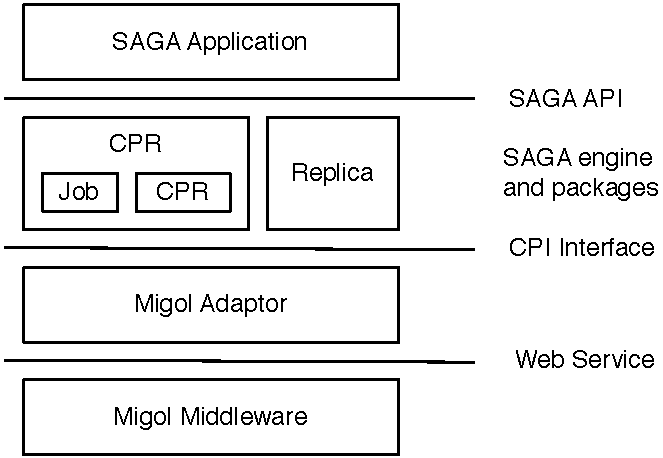
\includegraphics[width=0.6\textwidth]{saga-migol-layered}
%   \caption{\small \bf SAGA Adaptor for Migol infrastructure}
%   \label{fig:saga-migol-layered}
% \end{figure}  


% \section{Experiences with a Large-Scale Task-Farming Application in the LONI Grid}
% \label{sec:exp}       
% 
%         
% %do we use checkpoints or do we automatically restart the task
% Figure~\ref{fig:saga-taskfarming} gives an overview about the task farming scenario. All tasks are
% distributed using a script and Migol's Job Broker Service.
% %  Each worker will compute a certain 
% % variation of the graph network. Depending on the graph size, the runtime of a single task  can 
% % be as high as \textbf{TODO}  days. 
% To enable the monitoring of a tasks, each task must initialize a \texttt{saga::session} object 
% before starting the computation.  Then, the Migol adaptor starts and registers the monitoring endpoint. 
% %TODO what is the task size/runtime of a single task
% The MRS can now monitor the application.  For error detection we use a timeout of 5 minutes.
% \begin{figure}[t]
%     \centering
%         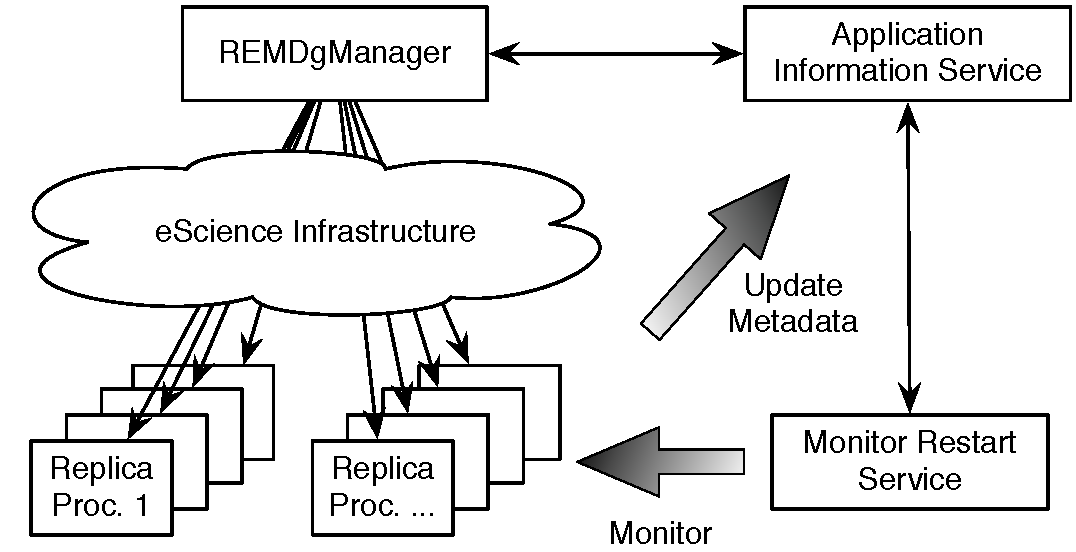
\includegraphics[width=\textwidth]{saga-taskfarming}
%     \caption{\small \bf Fault-Tolerant Task Farming Scenario}
%     \label{fig:saga-taskfarming}
% \end{figure}
% 
% 
% 
% 
%   
% 
% During the runtime, we simulate the failure of a number of worker
% processes.  The Migol MRS successfully detects the respective faults
% and recovers the worker nodes correctly. Even with a high failure
% rate, we were able to obtain the results of our computation.
